% Section 6.2, source PDF 78-90 / printed 68-80. Source-aligned staging, not yet accepted.
% block: exterior-calculus-section-heading page:78 type:section
\subsection{{外微积分}}\label{sec:exterior-calculus}

% block: exterior-calculus-fields pages:78,79 type:ordinary-paragraph
{向量微积分的主要研究对象是在区域 $\Omega\subset\mathbb R^n$ 上定义的函数 $\Omega\to\mathbb R$ 和向量场 $\Omega\to\mathbb R^n$. 在 $\mathbb R^n$ 上的外微积分中, 主要对象是微分 $k$-形式, 即函数 $\Omega\to\operatorname{Alt}^k\mathbb R^n$. 特别地, 它包含函数和向量场的情形. 事实上, 如前所见, 可以用两种不同而自然的方式将向量微积分中的函数看作微分形式 (或者是 $0$-形式, 或者是 $n$-形式), 类似地, 向量场可以与 $1$-形式或 $(n-1)$-形式等同. 这种在向量微积分中丢失的区别, 恰恰成为外微积分的优点. Maxwell 写道, "物理向量量可以分为两类, 一类参照线来定义, 另一类则参照面积来定义" \BookCite{58}, 说的就是这一点. 在更高维中还会出现其他类型的场. 例如, 四维中的微分 $2$-形式是具有六个独立分量的场 (即 $4\times4$ 反对称矩阵中独立分量的个数).}

% block: exterior-calculus-manifold-generality page:79 type:ordinary-paragraph
{实际上, 若采取更一般的观点, 允许区域 $\Omega$ 为任意流形 (有限维, 有边界或无边界, 并且足够光滑以使切空间有定义), 而不只是 $\mathbb R^n$ 中的开子集, 外微积分的展开就最为自然. 理论的很大一部分在这种一般程度下都成立, 只依赖区域的可微结构. 其他概念则需要附加结构: 内积 (即 Riemannian 流形), 或定向 (有定向流形), 或两者兼具; 使用特选基还可以简化某些公式. 当然, $\mathbb R^n$ 中的区域具有所有这些结构. 但像我们将要做的那样, 清楚记住何种运算需要何种结构, 很有启发性. 从实用角度看, 即使只关心求解 $\mathbb R^n$ 中的边值问题, 也不仅需要在定义微分方程的区域上使用微分形式, 还需要在其边界上使用; 边界是流形, 但不是 Euclidean 空间中的区域.}

% block: differential-forms-heading page:79 type:subsection
\subsubsection{{微分形式}}\label{subsec:differential-forms}

% block: tangent-bundle-sections page:79 type:ordinary-paragraph
{设 $\Omega$ 是维数为 $n$ 的流形. 在每个点 $x\in\Omega$ 处, 切空间 $T_x\Omega$ 是维数为 $n$ 的向量空间; 所有满足 $x\in\Omega$ 和 $v\in T_x\Omega$ 的二元组 $(x,v)$ 的集合定义了切丛, 它是维数为 $2n$ 的流形. 此丛的一个\emph{截面}是从 $\Omega$ 到其切丛的函数, 为每个 $x\in\Omega$ 指定一个切向量 $v_x\in T_x\Omega$. 也就是说, 它是切向量场.}

% block: differential-form-bundle page:79 type:ordinary-paragraph
{应用上一节的外代数构造, 可以定义一个丛 (余切丛的第 $k$ 次外幂), 由满足 $\mu\in\operatorname{Alt}^kT_x\Omega$ 的二元组 $(x,\mu)$ 构成. \emph{微分 $k$-形式}就是此丛的一个截面, 即为每个 $x\in\Omega$ 指定 $\operatorname{Alt}^kT_x\Omega$ 中一个元素的函数. 因此, $\omega$ 为微分 $k$-形式意味着}
\[
\omega_x(v_1,\ldots,v_k)\in\mathbb R\quad\forall x\in\Omega,\ v_1,\ldots,v_k\in T_x\Omega,
\]
{其中对向量 $v_i$ 的依赖是多重线性且交错的. 通常还要求对 $x$ 的依赖具有某种光滑性, 具体程度随上下文而定. 当 $\Omega$ 确为 $\mathbb R^n$ 的子区域时, 可将所有切空间与 $\mathbb R^n$ 等同, 因而微分 $k$-形式就是函数 $\Omega\to\operatorname{Alt}^k\mathbb R^n$. 它可写为}
\begin{equation}\label{eq:differential-form-coordinates}
\omega=\sum_{1\leq\sigma_1<\cdots<\sigma_k\leq n}a_\sigma\,dx^{\sigma_1}\wedge\cdots\wedge dx^{\sigma_k},
\end{equation}
{其中系数 $a_\sigma$ 是 $\Omega$ 上的实值函数.}

% block: differential-form-space-notation page:79 type:ordinary-paragraph
{不需要强调所要求的精确光滑程度时, 将 $\Omega$ 上的微分 $k$-形式向量空间记为 $\Lambda^k(\Omega)$, 或简称 $\Lambda^k$. 需要强调时, 则在这一记号之前加上函数空间. 例如, $C\Lambda^k$ 表示连续微分形式空间, $C^1\Lambda^k$ 表示连续可微形式空间, 等等. 下面将引入具有不同指定光滑程度的空间的记号.}

% block: differential-form-pointwise-operations page:80 type:ordinary-paragraph
\medskip\noindent\textbf{{外积, 缩并, 内积, Hodge 星算子, 向量代理}}\par
{上一节讨论的交错多重线性形式上的代数运算, 可以逐点应用于微分形式. 例如, $\omega\in\Lambda^j$ 和 $\mu\in\Lambda^k$ 的外积是如下微分 $(j+k)$-形式:}
\[
(\omega\wedge\mu)_x=\omega_x\wedge\mu_x.
\]
{类似地, 若 $v$ 是 $\Omega$ 上的向量场且 $\omega\in\Lambda^k(\Omega)$, 则 $\omega\lrcorner v$ 是微分 $(k-1)$-形式. 为延拓需要内积的运算, 要求流形 $\Omega$ 是 Riemannian 流形, 即在每点 $x$ 处的 $T_x\Omega$ 上给定内积. 内积应光滑地依赖于 $x$, 即若 $v_x$ 和 $w_x$ 是光滑向量场, 则 $x\mapsto\langle v_x,w_x\rangle_{T_x\Omega}$ 应为 $\Omega$ 上的光滑函数 (确切的光滑程度仍由上下文决定). 一些代数运算还需要切空间 $T_x\Omega$ 的定向, 并假设在各点以一致方式指定了这些定向. 这要求流形可定向. 例如在 Möbius 带上就不可能做到. 在有定向 Riemannian 流形上, 存在唯一的体积 $n$-形式, 其特征是在每点 $x$ 处, 将 $T_x\Omega$ 的每组正向标准正交基映为值 $1$. 随后由 \eqref{eq:hodge-star-characterization} 逐点定义从 $\Lambda^k$ 到 $\Lambda^{n-k}$ 的 Hodge 星算子, 并可按下式计算 $L^2\Lambda^k(\Omega)$ 中的内积:}
\[
\langle\omega,\nu\rangle_{L^2\Lambda^k}=\int_\Omega\langle\omega,\nu\rangle\operatorname{vol}=\int_\Omega\omega\wedge\star\nu,\qquad\omega,\nu\in L^2\Lambda^k(\Omega).
\]
{逐点应用向量代理, 可将微分 $0$-形式和微分 $n$-形式与流形上的实值函数等同, 将微分 $1$-形式和微分 $(n-1)$-形式与切向量场等同.}

% block: smooth-pullback page:80 type:ordinary-paragraph
\begingroup\emergencystretch=1em
\medskip\noindent\textbf{{光滑映射下的拉回与迹}}\par
{若 $\phi:M\to N$ 是流形之间的可微映射, 则其导数 $\phi'(x)$ 是从 $T_xM$ 到 $T_{\phi(x)}N$ 的线性映射. 若 $\omega\in\Lambda^k(N)$, 则可由下式定义 $\Omega$ 上的微分 $k$-形式:}
\begin{equation}\label{eq:smooth-pullback-definition}
(\phi^*\omega)_x=\phi'(x)^*\omega_{\phi(x)},
\end{equation}
{其中右端使用了 \eqref{eq:linear-pullback-definition} 定义的代数拉回. 这就定义了光滑映射下微分形式的拉回 $\phi^*\omega\in\Lambda^k(M)$. 与代数情形一样, 拉回反变地作用并保持外积.}

\par\endgroup
% block: differential-trace-proxies pages:80,81 type:ordinary-paragraph
{子流形 $M$ 到另一流形 $N$ 的包含映射的拉回称为迹算子, 记为 $\operatorname{tr}:\Lambda^k(N)\to\Lambda^k(M)$. 对 $0$-形式, 它就是函数的限制. 包含映射在点 $x\in M$ 处的导数, 就是 $T_xM\subset T_xN$ 的包含映射. 这一事实结合 Section~\ref{subsec:alternating-form-operations} 末尾的计算, 给出了两种重要情形下用代理表示的迹公式. 若 $w$ 是 $N$ 上对应于某个 $1$-形式 $\omega\in\Lambda^1(N)$ 的向量场, 则 $M$ 上对应于 $\operatorname{tr}\omega\in\Lambda^1(M)$ 的向量场 $\bar w$ 由下式给出:}
\[
\bar w(x)=\pi w(x),\qquad x\in M,
\]
{其中 $\pi=\pi_{T_xM}:T_xN\to T_xM$ 是正交投影. 如果 $\dim M=\dim N-1$, 且向量场 $w$ 对应于 $\omega\in\Lambda^{\dim N-1}(N)$, 则 $\operatorname{tr}\omega$ 对应于 $M$ 上的标量函数 $\langle w,n\rangle$, 其中 $n$ 是 $M$ 在 $N$ 中适当定向的单位法向量.}

% block: coordinate-trace page:81 type:ordinary-paragraph
{当 $M=\mathbb R^{n-1}$, $N=\mathbb R^n$, 且包含映射为 $x\mapsto(0,x)$ 时, 可用坐标写出相应的迹算子. 若 $\omega$ 是 \eqref{eq:differential-form-coordinates} 给出的微分形式, 则}
\begin{equation}\label{eq:differential-trace-coordinates}
\operatorname{tr}\omega=\sum_{\{\sigma\mid\sigma_1>1\}}(\operatorname{tr}a_\sigma)\,dx^{\sigma_1}\wedge\cdots\wedge dx^{\sigma_k}.
\end{equation}
{右端 $\operatorname{tr}a_\sigma$ 中的迹算子是 $0$-形式的迹, 即在 $\mathbb R^{n-1}$ 上的限制.}

% block: exterior-derivative-heading page:81 type:subsection
\subsubsection{{外微分}}\label{subsec:exterior-derivative}

% block: exterior-derivative-definition page:81 type:ordinary-paragraph
{将 $\Lambda^k(\Omega)$ 映到 $\Lambda^{k+1}(\Omega)$ 的外微分, 是外微积分的基本算子. 当 $\Omega$ 是 $\mathbb R^n$ 中的区域时, 定义最为简单. 若 $\omega$ 是光滑微分 $k$-形式, $v_1,\ldots,v_k$ 是 $\mathbb R^n$ 中的 $k$ 个向量, 则 $\omega_x(v_1,\ldots,v_k)$ 是 $x$ 的可微函数, 并且关于这 $k$ 个向量是交错多重线性的. 若再给定向量 $v_0$, 则可将沿 $v_0$ 方向的方向导数 $\partial_{v_0}:=v_0\cdot\operatorname{grad}$ 应用于此函数, 得到依赖于 $x$ 和全部 $(k+1)$ 个向量的量. 它对每个向量的依赖是线性的, 但并不交错. 为得到 $(k+1)$-形式, 取其交错部分. 再乘以 $k+1$, 就得到外微分 $d\omega$:}
\[
(d\omega)_x(v_0,\ldots,v_k)=\sum_{j=0}^k(-)^j\partial_{v_j}\omega_x(v_0,\ldots,\widehat{v_j},\ldots,v_k).
\]

% block: exterior-derivative-coordinates page:81 type:ordinary-paragraph
{用 $\mathbb R^n$ 上的标准坐标, $\Lambda^k(\Omega)$ 的一般元素可写为}
\[
\omega=\sum_{1\leq\sigma_1<\cdots<\sigma_k\leq n}f_\sigma\,dx^{\sigma_1}\wedge\cdots\wedge dx^{\sigma_k},
\]
{其中系数 $f_\sigma$ 是 $\Omega$ 上的函数. 则}
\begin{equation}\label{eq:exterior-derivative-coordinates}
d\omega=\sum_\sigma\sum_{j=1}^n\frac{\partial f_\sigma}{\partial x^j}\,dx^j\wedge dx^{\sigma_1}\wedge\cdots\wedge dx^{\sigma_k}.
\end{equation}

% block: exterior-derivative-vector-calculus page:81 type:ordinary-paragraph
{例如当 $k=0$ 时, 有公式}
\[
df=\sum_{j=1}^n\frac{\partial f}{\partial x^j}\,dx^j.
\]
{将右端的 $1$-形式与向量场等同, 可见 $\mathbb R^n$ 上作用于 $1$-形式的外微分就是梯度算子. 类似的考虑表明, 作用于 $(n-1)$-形式的外微分可以与散度算子等同. 在三维中, 作用于 $1$-形式的外微分可视为从向量场到向量场的映射, 并可知它就是旋度算子. 因此, 此时整个 de Rham 复形 \eqref{eq:differential-forms-de-rham-complex} 都可用向量微积分的术语写成 \eqref{eq:vector-calculus-de-rham-complex}.}

% block: exterior-derivative-pullback-invariance page:82 type:ordinary-paragraph
{外微分的一个重要性质是, 它在拉回下不变. 若 $\phi:\Omega\to M$ 是从 $\mathbb R^n$ 的子区域到 $\mathbb R^m$ 的子区域的映射, 且 $\omega\in\Lambda^k(M)$, 则 $\phi^*\omega\in\Lambda^k(\Omega)$, 并有}
\begin{equation}\label{eq:exterior-derivative-pullback}
d\phi^*\omega=\phi^*d\omega.
\end{equation}
{若 $\phi$ 是两个同维区域之间的微分同胚, 则得到}
\begin{equation}\label{eq:exterior-derivative-chart-definition}
d\omega=(\phi^{-1})^*d\phi^*\omega.
\end{equation}
{当 $M$ 是流形而不是 Euclidean 空间中的区域时, 可用此公式定义 $d\omega$. 任选将某个 $\Omega\subset\mathbb R^n$ 映到 $M$ 的一个开集上的坐标图 $\phi$, 再用公式 \eqref{eq:exterior-derivative-chart-definition} 定义该开子集上的 $d\omega$. 由于 $M$ 被坐标图覆盖, 由此就定义了 $d\omega\in\Lambda^k(M)$. 由 \eqref{eq:exterior-derivative-pullback} 可知, 此定义不依赖坐标图的选取. 此外, 这种拉回不变性对流形之间的任意光滑映射都成立.}

% block: exterior-differential-leibniz page:82 type:ordinary-paragraph
{外微分的另一个基本性质是, 它是满足 $d\circ d=0$ 意义下的微分. 只需在 $\mathbb R^n$ 中的区域上验证这一点, 在那里由偏导数的交换性, 很容易从 \eqref{eq:exterior-derivative-coordinates} 得出结论. 同样重要的是 Leibniz 法则}
\begin{equation}\label{eq:exterior-leibniz-rule}
d(\omega\wedge\mu)=d\omega\wedge\mu+(-)^k\omega\wedge d\mu,\qquad\omega\in\Lambda^k(\Omega),\ \mu\in\Lambda^j(\Omega).
\end{equation}
{值得强调的是, 外微分的定义完全不涉及流形上的内积 (度量) 或定向. 任意流形上的微分 $k$-形式都可以微分, 得到微分 $(k+1)$-形式.}

% block: differential-form-integration-heading page:82 type:subsection
\subsubsection{{微分形式的积分}}\label{subsec:differential-form-integration}

% block: integration-orientation page:82 type:ordinary-paragraph
{微分 $k$-形式可以在有定向的 $k$ 维流形上积分, 得到实数. 注意, 形式次数必须与流形维数相同. 定义积分不需要流形上的度量或测度, 即使存在这些结构, 积分也与它们无关. 但定向确实重要. 改变定向就会改变积分的符号.}

% block: integration-parallelepiped-definition page:82 type:ordinary-paragraph
{为初步理解积分如何定义, 考虑由一点 $x\in\mathbb R^k$ 和 $k$ 个线性无关向量 $v_1,\ldots,v_k$ 确定的平行多面体 $P$, 如 Figure~\ref{fig:integration-parallelograms}(a). 若 $\omega$ 是 $P$ 上的常 $k$-形式, 则 $\omega$ 在 $P$ 上的积分就是 $\omega_x(v_1,\ldots,v_k)$. 若 $\omega$ 光滑但非常值, 则当平行多面体足够小时, 这将是积分的良好近似. 现在, 利用坐标图, 任意流形都可被一组小的切平行多面体任意精确地逼近, 如 Figure~\ref{fig:integration-parallelograms}(b) 所示. 然后在每个平行四边形上计算 $\omega$ 并相加, 得到积分近似值}
\[
\int_\Omega\omega\approx\sum_i\omega_{x^{(i)}}(v_1^{(i)},\ldots,v_n^{(i)}),
\]
{其中 $x^{(i)}$ 和 $v_j^{(i)}$ 是确定这些平行四边形的点和切向量. 取极限便得到 $\int_\Omega\omega$.}

% block: integration-parallelograms-figure page:83 type:figure
\begin{figure}[htbp]\centering
\includegraphics[page=83,trim=102bp 494bp 52bp 62bp,clip,width=.90\linewidth]{../input/source/Finite Element Exterior Calculus.pdf}
\caption{{(a) 由一点及该点处两个切向量确定的平行四边形. (b) 二维流形可由一组切平行四边形任意精确地逼近.}}\label{fig:integration-parallelograms}
\end{figure}

% block: integration-diffeomorphism-invariance page:83 type:ordinary-paragraph
{由定义容易得到, 积分在保定向微分同胚下不变. 即若 $\phi:M\to N$ 是 $n$ 维流形之间这样的微分同胚, 则}
\begin{equation}\label{eq:integration-pullback-invariance}
\int_M\phi^*\omega=\int_N\omega,\qquad\omega\in\Lambda^n(N).
\end{equation}
{特别地, 可以用坐标图将流形上的积分计算化为 $\mathbb R^n$ 的子区域上的积分, 大多数性质也能由此验证. 若 $\Omega$ 是这样的区域, 则 $\Omega$ 上的 $n$-形式可写为 $f(x^1,\ldots,x^n)\,dx^1\wedge\cdots\wedge dx^n$, 它的积分恰如记号}
\[
\int_\Omega f(x^1,\ldots,x^n)\,dx^1\wedge\cdots\wedge dx^n
\]
{所示 (即它等于函数 $f$ 在 $\Omega$ 上的 Lebesgue 积分). 更一般地, 若 $\Omega$ 是有定向 Riemannian 流形, 则 $\int_\Omega f\operatorname{vol}$ 等于 $f$ 关于相应 Riemannian 测度的积分.}

% block: integration-over-submanifold page:83 type:ordinary-paragraph
{若 $\omega$ 是 $n$ 维流形 $\Omega$ 上的 $k$-形式, $M$ 是 $\Omega$ 的有定向 $k$ 维子流形, 则 $\omega$ 在 $M$ 上的迹, 是 $k$ 维流形上的 $k$-形式, 因而可在 $M$ 上积分. 严格地说, 结果应写为 $\int_M\operatorname{tr}_M\omega$, 但通常简写为 $\int_M\omega$. 例如, 设 $M$ 是 $\mathbb R^n$ 中某个区域内的有定向曲线, $\omega$ 是该区域上的 $1$-形式. 可以将 $\omega$ 看作向量场, 此时 $\operatorname{tr}_M\omega$ 对应于向量场在曲线上的切向投影. 因此 $\int_M\omega$ 就是向量微积分中通常的曲线积分.}

% block: stokes-integration-by-parts-heading page:83 type:subsection
\subsubsection{{Stokes 定理与分部积分}}\label{subsec:stokes-integration-by-parts}

% block: stokes-theorem page:83 type:ordinary-paragraph
{外微积分的顶点是 Stokes 定理, 它是微积分基本定理的广泛推广. 在对紧致有定向 $n$ 维带边界流形 $\Omega$ 及微分形式 $\omega$ 施加相对温和的光滑性要求下, 该定理断言}
\[
\int_\Omega d\omega=\int_{\partial\Omega}\operatorname{tr}\omega,\qquad\omega\in\Lambda^{n-1}(\Omega).
\]

% block: stokes-boundary-orientation page:84 type:ordinary-paragraph
{同样, 陈述结果时通常不显式写出迹算子. 边界定向由流形的定向继承而来 (即边界某点处切空间的一组正向基, 是在前面添上该点的外法向量后, 成为 $\Omega$ 的正向基的那组基).}
{在此等式中将 $\omega$ 替换为 $\omega\wedge\mu$, 并使用 Leibniz 法则 \eqref{eq:exterior-leibniz-rule}, 得到分部积分公式:}
\begin{equation}\label{eq:differential-forms-integration-by-parts}
\begin{gathered}
\int_\Omega d\omega\wedge\mu=(-)^{k+1}\int_\Omega\omega\wedge d\mu+\int_{\partial\Omega}\operatorname{tr}\omega\wedge\operatorname{tr}\mu,\\
\omega\in\Lambda^k(\Omega),\ \mu\in\Lambda^{n-k-1}(\Omega),
\end{gathered}
\end{equation}
{它对足够光滑的形式成立 (下面将研究所需的光滑性). 使用边界上的 Hodge 星算子, 可将边界积分写为内积 $\langle\star\operatorname{tr}\omega,\operatorname{tr}\mu\rangle_{L^2\Lambda^{n-k-1}(\partial\Omega)}$.}

% block: piola-application-heading page:84 type:subsection
\subsubsection{{一个应用例子}}\label{subsec:piola-application}

% block: piola-application-derivation page:84 type:ordinary-paragraph
{在继续之前, 先用外微积分框架导出向量微积分中的一个结果, 它在混合有限元的发展中起着重要作用. (该结果的二维表述可参见例如 [\BookNumber{19}, Lemma 2.1.6].) 设 $p:\Omega\to\mathbb R$ 和 $v:\Omega\to\mathbb R^3$ 分别是 $\mathbb R^3$ 中区域 $\Omega$ 上的标量场和向量场, 考虑内积 $(p,\operatorname{div}v)_{L^2(\Omega)}$. 将散度视为 $2$-形式的外微分, 令 $\nu=v^1dx^2\wedge dx^3-v^2dx^1\wedge dx^3+v^3dx^1\wedge dx^2$ 为向量代理为 $v$ 的微分 $2$-形式. 则 $d\nu=(\operatorname{div}v)\operatorname{vol}$, 且 $(p,\operatorname{div}v)_{L^2(\Omega)}=\int_\Omega p\wedge d\nu$, 其中右端积分是微分形式意义下的积分. 再设 $\phi:\widehat\Omega\to\Omega$ 是保定向微分同胚, 应用积分 \eqref{eq:integration-pullback-invariance}, 外积 \eqref{eq:linear-pullback-wedge} 和外微分 \eqref{eq:exterior-derivative-pullback} 的拉回不变性, 将 $\Omega$ 上的积分变为 $\widehat\Omega$ 上的积分:}
\[
\int_\Omega p\wedge d\nu=\int_{\widehat\Omega}\phi^*(p\wedge d\nu)=\int_{\widehat\Omega}\phi^*p\wedge\phi^*d\nu=\int_{\widehat\Omega}\phi^*p\wedge d\phi^*\nu.
\]
{由场的拉回定义 \eqref{eq:smooth-pullback-definition}, 以及 Table~\ref{tab:exterior-algebra-r3} 底部给出的线性映射拉回公式, 可知 $\phi^*p=\hat p:=p\circ\phi$, 而 $\phi^*\nu$ 的代理场为向量场}
\[
\hat v=(\det\phi')(\phi')^{-1}(v\circ\phi):\widehat\Omega\to\mathbb R^3.
\]
{向量场 $\hat v$ 称为 $v$ 的 \emph{Piola 变换}. 可见, Piola 变换自然地作为 $2$-形式的拉回出现, 因而满足关键性质}
\[
(p,\operatorname{div}v)_{L^2(\Omega)}=(\hat p,\operatorname{div}\hat v)_{L^2(\widehat\Omega)}.
\]

% block: differential-forms-l2-heading page:84 type:subsection
\subsubsection{{微分形式的 $L^2$ 理论}}\label{subsec:differential-forms-l2-theory}

% block: differential-forms-l2-introduction page:84 type:ordinary-paragraph
{本节假设 $\Omega$ 为光滑紧致 $n$ 维有定向 Riemannian 流形, 可以有边界或无边界; 将外微分 $d=d^k$ 看作从 $L^2\Lambda^k(\Omega)$ 到 $L^2\Lambda^{k+1}(\Omega)$ 的稠定闭无界算子, 它们组合构成 $L^2$ de Rham 复形. 我们将证明外微分算子都具有闭像, 并计算其伴随.}

% block: l2-techniques-and-inner-product page:85 type:ordinary-paragraph
{这些技巧与 Section~\ref{sec:vector-operators-adjoints} 中处理 $\mathbb R^3$ 内区域这一特殊情形所用的技巧完全平行.}

{由于假设给定了定向和 Riemannian 结构, Hodge 星算子是良定义的. 由 \eqref{eq:hodge-star-inner-product}, 两个 $k$-形式的 $L^2$ 内积为}
\[
\langle\omega,\mu\rangle_{L^2\Lambda^k}=\int_\Omega\langle\omega,\mu\rangle\operatorname{vol}=\int_\Omega\omega\wedge\star\mu,\qquad\omega,\mu\in\Lambda^k(\Omega).
\]
{在不易混淆时, 可以从内积的下标中省略 $\Lambda^k$, 或将下标全部省略.}

% block: codifferential-definition page:85 type:ordinary-paragraph
{\emph{余微分}算子定义为 $\delta=\pm\star d\star$. 符号由要求 $\delta=\delta^k:\Lambda^k\to\Lambda^{k-1}$ 满足下式来确定:}
\[
\star\delta\omega=(-)^kd\star\omega,\qquad\omega\in\Lambda^k.
\]
{在 \eqref{eq:differential-forms-integration-by-parts} 中令 $\mu=\star\nu$, 并使用 $\delta$ 的这个定义, 得到分部积分公式的第二种形式:}
\[
\begin{gathered}
\langle d\omega,\nu\rangle=\langle\omega,\delta\nu\rangle+\int_{\partial\Omega}\operatorname{tr}\omega\wedge\operatorname{tr}\star\nu,\\
\omega\in\Lambda^k,\ \nu\in\Lambda^{k+1}.
\end{gathered}
\]
{此公式表明 $\delta$ 是 $d$ 的形式伴随, 这解释了其定义中的符号选取.}

% block: distributional-exterior-derivative page:85 type:ordinary-paragraph
{若 $\omega\in L^2\Lambda^k(\Omega)$ 且 $\mu\in L^2\Lambda^{k+1}(\Omega)$, 则方程 $d\omega=\mu$ 在分布意义下有意义, 即意味着}
\[
\langle\omega,\delta\nu\rangle=\langle\mu,\nu\rangle,\qquad\nu\in C_0^\infty\Lambda^{k+1}(\Omega).
\]
{于是将 $H\Lambda^k(\Omega)$ 定义为满足 $d\omega\in L^2\Lambda^{k+1}(\Omega)$ 的 $\omega\in L^2\Lambda^k(\Omega)$ 的集合, 即存在这样的 $\mu\in L^2\Lambda^{k+1}(\Omega)$. 换言之, 将 $d$ 定义为从 $L^2\Lambda^{k+1}$ 到 $L^2\Lambda^k$ 的算子 $\delta$ 的伴随, 后者的定义域取为 $C_0^\infty\Lambda^{k+1}(\Omega)$. 作为稠定算子的伴随, 这样定义的 $d$ 是闭算子. 它在 $L^2\Lambda^k$ 中也稠定, 因为显然 $C_0^\infty\Lambda^k(\Omega)$ 包含于 $H\Lambda^k(\Omega)$, 并且在 $L^2\Lambda^k(\Omega)$ 中稠密. 由于 $d$ 是一阶线性微分算子, 有 $H^1\Lambda^k(\Omega)\subset H\Lambda^k(\Omega)$ (当 $k=0$ 时, 两者相等, 都与标准 Sobolev 空间 $H^1(\Omega)$ 一致). 还将使用 $C^\infty\Lambda^k(\bar\Omega)$ 在 $H\Lambda^k(\Omega)$ 中稠密这一事实. 其证明与通常 Sobolev 空间的证明一样, 使用磨光法 [\BookNumber{41}, Section 5.3.3].}

% block: l2-manifold-de-rham-complex page:85 type:ordinary-paragraph
{Hilbert 空间 $L^2\Lambda^k(\Omega)$ 和从 $L^2\Lambda^k(\Omega)$ 到 $L^2\Lambda^{k+1}(\Omega)$, 定义域为 $H\Lambda^k(\Omega)$ 的闭无界算子 $d^k$, 构成一个 Hilbert 复形, 即流形上的 $L^2$ de Rham 复形:}
\[
\begin{gathered}
0\to L^2\Lambda^0(\Omega)\xrightarrow{(d^0,H\Lambda^0)}L^2\Lambda^1(\Omega)\xrightarrow{(d^1,H\Lambda^1)}\cdots\\
\xrightarrow{(d^{n-1},H\Lambda^{n-1})}L^2\Lambda^n(\Omega)\to0.
\end{gathered}
\]
{为使表达简洁些, 可以简写为}
\begin{equation}\label{eq:l2-manifold-de-rham-complex}
0\to L^2\Lambda^0\xrightarrow{(d,H\Lambda)}L^2\Lambda^1\xrightarrow{(d,H\Lambda)}\cdots\xrightarrow{(d,H\Lambda)}L^2\Lambda^n\to0
\end{equation}
{或者只给出定义域复形}
\begin{equation}\label{eq:manifold-de-rham-domain-complex}
0\to H\Lambda^0\xrightarrow{d}H\Lambda^1\xrightarrow{d}\cdots\xrightarrow{d}H\Lambda^n\to0.
\end{equation}

% block: forms-trace-extension-introduction pages:85,86 type:ordinary-paragraph
{现在考察分部积分公式 \eqref{eq:differential-forms-integration-by-parts}, 建立它对 $\omega$ 和 $\mu$ 成立的条件. 它当然对光滑的 $\omega$ 和 $\mu$ 成立, 因而由稠密性, 对 $\omega\in H^1\Lambda^k$, $\mu\in H^1\Lambda^{n-k-1}$ 成立. 为进一步推广, 现在证明迹算子可延拓为 $H\Lambda^k(\Omega)$ 上取值于 $H^{-1/2}\Lambda^k(\partial\Omega)$ 的有界算子. 完成后, 就可将 \eqref{eq:differential-forms-integration-by-parts} 延拓到一个形式属于 $H\Lambda$, 另一个属于 $H^1\Lambda$ 的情形. (除非至少一个形式的迹为零, 否则不能允许两个形式都在 $H\Lambda$ 中, 因为那样边界积分就没有意义.)}

% block: forms-zero-trace-identity page:86 type:ordinary-paragraph
{由定义,}
\[
\langle d\omega,\nu\rangle-\langle\omega,\delta\nu\rangle=0,\qquad\omega\in H\Lambda^k,\ \nu\in C_0^\infty\Lambda^{k+1}.
\]
{等价地, 代入 $\mu=\star\nu$ 后,}
\[
\int d\omega\wedge\mu-(-)^{k+1}\int\omega\wedge d\mu=0,\qquad\omega\in H\Lambda^k,\ \mu\in C_0^\infty\Lambda^{n-k-1}.
\]
{对固定的 $\omega\in H\Lambda^k$, 左端定义了作用于 $\mu\in H\Lambda^{n-k-1}$ 的有界线性泛函. 将 $\mathring H\Lambda^{n-k-1}$ 定义为 $C_0^\infty\Lambda^{n-k-1}$ 在 $H\Lambda^{n-k-1}$ 中的闭包, 则该等式对所有 $\omega\in H\Lambda^k$, $\mu\in\mathring H\Lambda^{n-k-1}$ 成立.}

% block: forms-lipschitz-boundary-charts page:86 type:ordinary-paragraph
{为继续研究迹映射, 假设边界是 Lipschitz 的, 即可用 $\Omega$ 的开集 $U$ 覆盖它, 这些开集通过 Lipschitz 坐标图映到半球 $B=\{\,x\in\mathbb R^n\mid|x|=1,\ x^n\geq0\,\}$, 且 $U\cap\partial\Omega$ 映到 $B_0:=B\cap\{x^n=0\}$. 随后可将空间 $H^1\Lambda^k(U)$ 和 $H^{1/2}\Lambda^k(U\cap\partial\Omega)$ 分别定义为 $B$ 和 $B_0$ 上相应空间的拉回, 再通过单位分解将这些空间拼接起来, 定义空间 $H^1\Lambda^k(\Omega)$ 和 $H^{1/2}\Lambda^k(\partial\Omega)$.}

% block: forms-h1-trace-surjectivity page:86 type:theorem
\Needspace{6\baselineskip}
\begin{Theorem}\label{thm:forms-h1-trace-surjectivity}
{$k$-形式上的迹映射将 $H^1\Lambda^k(\Omega)$ 映到 $H^{1/2}\Lambda^k(\partial\Omega)$ 上.}
\end{Theorem}

% block: forms-h1-trace-surjectivity-proof page:86 type:proof
\begin{Proof}
{由前面的讨论, 只需证明 $\Omega$ 是 $\mathbb R^n$ 中的半球 $B$, 且在 $B_0$ 上计算迹的情形. 这由迹的公式 \eqref{eq:differential-trace-coordinates}, 以及标量迹 $H^1(B)\to H^{1/2}(B_0)$ 的满射性得出.}
\end{Proof}

% block: forms-trace-duality page:86 type:ordinary-paragraph
{像 Lemma~\ref{prop:trace-functional-representation} 的证明那样应用对偶性 Lemma~\ref{lem:dual-surjection-annihilator}, 可知迹映射的对偶是有界线性单射, 其像是迹映射零空间的零化子, 从而得到下述推论.}

% block: forms-trace-functional-representation page:86 type:corollary
\Needspace{8\baselineskip}
\begin{Corollary}\label{cor:forms-trace-functional-representation}
{若 $L:H^1\Lambda^k(\Omega)\to\mathbb R$ 是有界线性泛函, 且只要 $\operatorname{tr}\omega=0$ 就有 $L\omega=0$, 则存在唯一 $g\in H^{-1/2}\Lambda^k(\partial\Omega)$, 使得}
\[
L\omega=\langle g,\operatorname{tr}\omega\rangle,\qquad\omega\in H^1\Lambda^k(\Omega).
\]
{此外, $\|g\|_{H^{-1/2}\Lambda^k(\partial\Omega)}\leq c\|L\|_{H^1\Lambda^k(\Omega)'}$.}
\[
L\omega=\int_{\partial\Omega}\operatorname{tr}\omega\wedge h,\qquad\omega\in H^1\Lambda^k(\Omega).
\]
\end{Corollary}

% block: forms-trace-representation-last-statement page:86 type:ordinary-paragraph
{最后一个陈述只需取 $h=\star g$, 其中 Hodge 星算子位于边界上 (积分通过稠密延拓而有意义).}

% block: forms-weak-trace-construction page:87 type:ordinary-paragraph
{现在, 若 $\mu\in H\Lambda^{n-k-1}$, 且 $\omega\in H^1\Lambda^k$ 满足 $\operatorname{tr}\omega=0$, 则有}
\[
\int_\Omega d\omega\wedge\mu-(-)^k\int_\Omega\omega\wedge d\mu=0.
\]
{(若 $\mu\in H^1\Lambda^{n-k-1}$, 这当然成立, 再由稠密性延拓到 $\mu\in H\Lambda$.) 因此, 对任意这样的 $\mu$, 可将该推论应用于泛函}
\[
L_\mu\omega:=\int_\Omega d\omega\wedge\mu-(-)^k\int_\Omega\omega\wedge d\mu
\]
{并得出存在唯一 $\gamma\mu\in H^{-1/2}\Lambda^{n-k-1}(\partial\Omega)$, 使得}
\[
\int_\Omega d\omega\wedge\mu-(-)^k\int_\Omega\omega\wedge d\mu=\int_{\partial\Omega}\operatorname{tr}\omega\wedge\gamma\mu,\qquad\omega\in H^1\Lambda^k.
\]
{显然, 若 $\mu$ 光滑, 例如属于 $H^1\Lambda^{n-k-1}$, 则 $\gamma\mu=\operatorname{tr}\mu$. 由此将 $H^1\Lambda^{n-k-1}$ 上的迹算子延拓为有界算子}
\[
H\Lambda^{n-k-1}(\Omega)\to H^{-1/2}\Lambda^{n-k-1}(\partial\Omega).
\]
{以下将此延拓算子记为 $\operatorname{tr}$ 而不是 $\gamma$. 概括为下述定理.}

% block: forms-weak-trace-theorem page:87 type:theorem
\Needspace{8\baselineskip}
\begin{Theorem}\label{thm:forms-weak-trace-extension}
{在 $H^1\Lambda^k(\Omega)$ 上的迹映射可延拓为有界线性算子 $\operatorname{tr}:H\Lambda^k(\Omega)\to H^{-1/2}\Lambda^k(\partial\Omega)$. 此外, 有分部积分公式的延拓版本:}
\begin{equation}\label{eq:forms-extended-integration-by-parts}
\begin{gathered}
\int_\Omega d\omega\wedge\mu=(-)^k\int_\Omega\omega\wedge d\mu+\int_{\partial\Omega}\operatorname{tr}\mu\wedge\operatorname{tr}\omega,\\
\omega\in H^1\Lambda^k,\ \mu\in H\Lambda^{n-k-1}.
\end{gathered}
\end{equation}
\end{Theorem}

% block: forms-final-results-introduction page:87 type:ordinary-paragraph
{本章最后再给出几个有用的结果.}

% block: forms-zero-trace-characterization page:87 type:theorem
\Needspace{6\baselineskip}
\begin{Theorem}\label{thm:forms-zero-trace-characterization}
{空间 $\mathring H\Lambda^k(\Omega)$ 定义为 $C_0^\infty\Lambda^k(\Omega)$ 在 $H\Lambda^k$ 中的闭包, 它由所有满足 $\operatorname{tr}\omega=0$ 的 $\omega\in H\Lambda^k(\Omega)$ 构成.}
\end{Theorem}

% block: forms-zero-trace-characterization-proof page:87 type:proof
\begin{Proof}
{证明与通常 Sobolev 空间的情形一样, 使用单位分解和边界拉平, 并结合半空间迹的直接构造. 见 [\BookNumber{41}, Theorem 5.5.2].}
\end{Proof}

% block: boundary-manifold-de-rham-complex page:87 type:ordinary-paragraph
{算子 $(d^k,\mathring H\Lambda^k)$, 即以此较小空间为定义域的算子 $d^k$, 给出了带边界条件的 de Rham 复形, 它是另一个 Hilbert 复形:}
\begin{equation}\label{eq:boundary-manifold-de-rham-complex}
0\to L^2\Lambda^0\xrightarrow{(d,\mathring H\Lambda)}L^2\Lambda^1\xrightarrow{(d,\mathring H\Lambda)}\cdots\xrightarrow{(d,\mathring H\Lambda)}L^2\Lambda^n\to0.
\end{equation}

% block: codifferential-l2-domain page:87 type:ordinary-paragraph
{算子 $\delta$ 的 $L^2$ 理论可以仿照刚才对 $d$ 的处理得到. 或者, 也可以通过 Hodge 星算子, 由 $d$ 的性质导出 $\delta$ 的性质. 可将 $\delta$ 看作 $L^2\Lambda^k$ 上的稠定闭算子, 定义域为}
\[
H^*\Lambda^k(\Omega)=\{\,\omega\in L^2\Lambda^k\mid\delta\omega\in L^2\Lambda^{k-1}\,\}=\star H\Lambda^{n-k}(\Omega).
\]

% block: codifferential-boundary-domain page:88 type:ordinary-paragraph
{由 Theorem~\ref{thm:forms-weak-trace-extension}, 算子 $\operatorname{tr}\star$ 有界地作用于}
\[
H^*\Lambda^k(\Omega)\to H^{-1/2}\Lambda^{n-k}(\partial\Omega).
\]
{$C_0^\infty\Lambda^k$ 在 $H^*\Lambda^k$ 中的闭包为}
\[
\mathring H^*\Lambda^k=\{\,\omega\in H^*\Lambda^k\mid\operatorname{tr}\star\omega=0\,\}.
\]
{以此空间为 $\delta$ 的定义域, 就得到另一个算子. 下述定理概括了这些算子的伴随.}

% block: exterior-codifferential-adjoints page:88 type:theorem
\Needspace{8\baselineskip}
\begin{Theorem}\label{thm:exterior-codifferential-adjoints}
{下列各算子的伴随为}
\begin{enumerate}
\item{$(d,H\Lambda^k)$ 的伴随为 $(\delta,\mathring H^*\Lambda^{k+1})$;}
\item{$(d,\mathring H\Lambda^k)$ 的伴随为 $(\delta,H^*\Lambda^{k+1})$;}
\item{$(\delta,H^*\Lambda^{k+1})$ 的伴随为 $(d,\mathring H\Lambda^k)$;}
\item{$(\delta,\mathring H^*\Lambda^{k+1})$ 的伴随为 $(d,H\Lambda^k)$.}
\end{enumerate}
\end{Theorem}

% block: manifold-complex-compactness page:88 type:ordinary-paragraph
{对前两个算子各自都有相应的 Hilbert 上链复形, 即分别为不带和带边界条件的 de Rham 上链复形 \eqref{eq:l2-manifold-de-rham-complex} 和 \eqref{eq:boundary-manifold-de-rham-complex}. (最后两个算子类似地构成 Hilbert 链复形, 除指标变化外, 它们与相应的 de Rham 复形本质上相同.) 由 Section~\ref{sec:l2-de-rham-complex} 讨论的 Picard 的结果可知, 这些复形各自都满足紧性性质, 从而所有算子都具有闭像, 所有复形都是 Fredholm 的. 知道伴随后, 就可写出与这两个复形相伴的 Hodge Laplace 边值问题的强表述. 对每一个复形, 微分方程都是 Hodge Laplace 方程}
\[
(d^{k-1}\delta_k+\delta_{k+1}d^k)u=f
\]
{或者省略上下标, 写为 $(d\delta+\delta d)u=f$. 对复形 \eqref{eq:l2-manifold-de-rham-complex}, 由要求 $u$ 和 $du$ 必须属于定义域 $d^*$ 所蕴含的边界条件为}
\[
\operatorname{tr}\star u=0,\qquad\operatorname{tr}\star du=0\quad\text{on }\partial\Omega.
\]

% block: manifold-magnetic-electric-conditions page:88 type:ordinary-paragraph
{这些边界条件在三维中的解释, 已在 Section~\ref{sec:hodge-r3} 中讨论, 并概括于 Table~\ref{tab:hodge-r3-boundary-conditions}. 对 $k=0$, 即标量 Laplacian 的情形, 第一个边界条件为空条件, 第二个则说明 $(\operatorname{grad}u)\cdot n=0$, 给出 \emph{Neumann 边界条件}. 对 $k=1$, 它们是磁边界条件; 对 $k=2$, 是电边界条件; 对 $k=3$, 它们施加 Dirichlet 边界条件.}

% block: manifold-essential-boundary-conditions page:88 type:ordinary-paragraph
{还可以考虑带边界条件的复形 \eqref{eq:boundary-manifold-de-rham-complex}. 此时边界条件是本质的, 来自要求 $u$ 属于 $\mathring H\Lambda^k$, $\sigma$ 属于 $\mathring H\Lambda^{k-1}$:}
\[
\operatorname{tr}u=0,\qquad\operatorname{tr}\delta u=0\quad\text{on }\partial\Omega.
\]
{它们在三维中的解释概括于 Table~\ref{tab:hodge-r3-relative-boundary-conditions}.}

% block: exterior-calculus-summary-heading page:89 type:ordinary-paragraph
\Needspace{36\baselineskip}
\begin{tcolorbox}[enhanced,breakable,colback=KuangNei,frame hidden,boxrule=0pt,sharpish corners,before skip=10pt,after skip=10pt]
\refstepcounter{booksummary}\label{box:exterior-calculus-summary}
\noindent\textbf{Box~\thebooksummary:} {Chapter~\ref{chap:exterior-calculus} 外微积分内容摘要.}\par

% block: exterior-summary-algebra page:89 type:ordinary-paragraph
{对 $n$ 维向量空间 $V$, $V$ 上交错 $k$-线性形式的空间 $\operatorname{Alt}^kV$ 具有维数 $\binom nk$. 其上具有多种代数运算:}
\begin{itemize}
\item{\emph{楔积}: $\wedge:\operatorname{Alt}^kV\times\operatorname{Alt}^jV\to\operatorname{Alt}^{k+j}V$.}
\item{\emph{缩并}: $\lrcorner:\operatorname{Alt}^kV\times V\to\operatorname{Alt}^{k-1}V$.}
\item{由线性映射 $L:V\to W$ 诱导的\emph{拉回} $L^*:\operatorname{Alt}^kW\to\operatorname{Alt}^kV$.}
\item{由 $V$ 上的内积诱导的 $\operatorname{Alt}^kV$ 上的\emph{内积}.}
\item{\emph{体积形式} $\operatorname{vol}$, 即张成 $\operatorname{Alt}^nV$ 的典范单位范数元素 $\operatorname{vol}$ (需要 $V$ 上的内积和定向).}
\item{\emph{Hodge 星算子}, 即典范等距映射 $\star:\operatorname{Alt}^kV\to\operatorname{Alt}^{n-k}V$ (需要 $V$ 上的内积和定向).}
\item{\emph{代理}: $\operatorname{Alt}^0V$ 和 $\operatorname{Alt}^nV$ 与 $\mathbb R$ 典范同构, $\operatorname{Alt}^1V$ 和 $\operatorname{Alt}^{n-1}V$ 与 $V$ 典范同构.}
\end{itemize}

% block: exterior-summary-differentiation page:89 type:ordinary-paragraph
{流形上的\emph{微分 $k$-形式}在每一点指定切空间的 $\operatorname{Alt}^k$ 中的一个元素. 上述所有运算都可推广到微分形式. 此外, 微分 $k$-形式 $\omega$ 具有外微分 $d\omega$, 它是微分 $(k+1)$-形式. 外微分满足 $d\circ d=0$ 和 Leibniz 法则:}
\[
d(\omega\wedge\mu)=d\omega\wedge\mu+(-)^k\omega\wedge d\mu,\qquad\omega\in\Lambda^k(\Omega),\ \mu\in\Lambda^j(\Omega).
\]

% block: exterior-summary-integration page:89 type:ordinary-paragraph
{微分 $n$-形式可以在有定向 $n$ 维流形上积分, 并满足 Stokes 定理}
\[
\int_\Omega d\omega=\int_{\partial\Omega}\operatorname{tr}\omega,
\]
{其中迹算子 $\operatorname{tr}$ 是包含映射 $\partial\Omega\subset\Omega$ 的拉回.}

% block: exterior-summary-hilbert-complex page:89 type:ordinary-paragraph
{在光滑紧致有定向的带边界 Riemannian 流形上, 分部积分公式 \eqref{eq:forms-extended-integration-by-parts} 成立. 在那里, 可以将外微分看作从 $L^2\Lambda^k\to L^2\Lambda^{k+1}$ 的无界算子, 定义域为 $H\Lambda^k$. \emph{$L^2$ de Rham 复形}是闭 Hilbert 复形, 其定义域复形为}
\[
0\to H\Lambda^0\xrightarrow{d}H\Lambda^1\xrightarrow{d}\cdots\xrightarrow{d}H\Lambda^n\to0.
\]
{伴随复形的定义域复形为}
\[
0\leftarrow\mathring H^*\Lambda^0\xleftarrow{\delta}\mathring H^*\Lambda^1\xleftarrow{\delta}\cdots\xleftarrow{\delta}\mathring H^*\Lambda^n\leftarrow0,
\]
{其中 $\delta=\pm\star d\star$ 是余微分. 也可以在 de Rham 复形中加入边界条件, 此时它们就不出现在伴随复形中.}
\end{tcolorbox}

% Original PDF 90 is a blank production leaf with printer calibration/registration marks,
% not a missing mathematical paragraph. It is retained unchanged in the source PDF.
